\chapter{VANS macroscopic applications}

\chapquote{I had to make some optimistic assumptions to meet the revenue target. In week three, we’re visited by an alien named D’utox Inag who offers to share his advanced technology.}{}{Dilbert comics by Scott Adams}

\section{Introduction}

bla bla bla .....


\section{Cavity geometry and condition}

The problem we want to solve is the classical closed cavity in three dimensions.
The cavity is a square with size $L$, the lateral and bottom walls are fixed and a constant velocity $U^{top}$ is specified at the top side.
On the front and back side we apply periodic boundary condition since the simulation domain has a depth equal to $\ell$.
A rigid porous media made by fibers is present at the bottom of the cavity and his vertical extension is equal to $h$.
The \textit{reference elementary volume} of the porous medium is a cubic cell of size $\ell$ with a cylinder with diameter $d$ at his center (regular arrangement of the fibers).
The permeability of the medium $\varepsilon$ is equal to 0.8 and the microscopic length scale has been chosen in order to have 50 fibers in the cavity.

\begin{figure}[h]
\centering
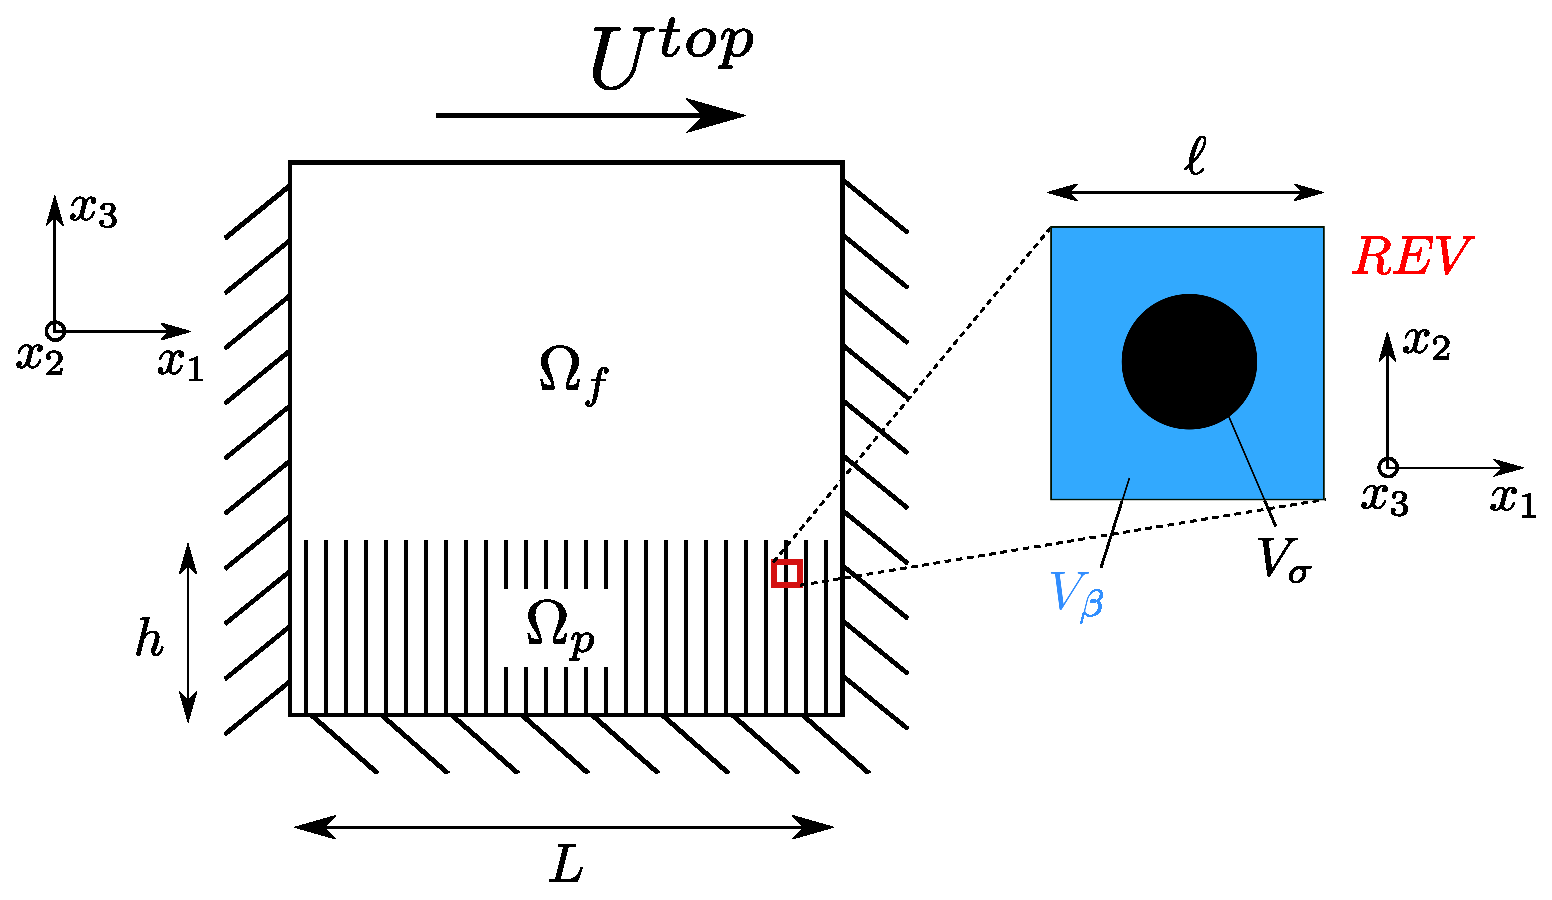
\includegraphics[width=0.7\linewidth]{chapter_5/figure/cavity_draw.eps}
\caption{Schematics of the closed cavity 2D problem. The porous medium internal structure is depicted in the zoom on the right side in which the REV geometry is showed.}
\label{fig:geom}
\end{figure}

\begin{itemize}
	\item $L$: side of the cavity, also the macroscopic length scale
	\item $h$: vertical extension of the fibers from the bottom of the cavity 
	\item $\ell$: side of the cubic REV, also the microscopic length scale
	\item $d$: diameter of the cylindrical fiber
	\item $V_{\beta}$: volume of the fluid inside the REV
	\item $V_{\sigma}$: volume of the solid inside the REV
	\item $\varepsilon$: porosity of the medium $\varepsilon = \dfrac{V_{\beta}}{V_{\sigma} +V_{\beta}}$
	\item $\eta$: length scale ratio $\eta = \dfrac{\ell}{L}$
	\item $Re$: Reynolds number of the cavity $Re = \dfrac{U^{top} L}{\nub}$
\end{itemize}

The overall domain has the size $L \, \times \, \ell \, \times \, L$ respectively in the $x_1$, $x_2$ and $x_3$ directions.
So we solve a weakly three dimensional problem since we include only one REV in the $x_2$ axes and we impose periodic boundary condition in the same direction.
But this is a fair assumption since the Reynolds number is small and we do not expect any 3D structure in the flow.

\subsection{Microscopic DNS Equations and Algorithm}

In this approach we (Giuseppe) have solved the incompressible Navier-Stokes equations in the three dimensional case \eqref{eq:mom}, \eqref{eq:cont} with the boundary conditions \eqref{eq:noslip},\eqref{eq:presspper},\eqref{eq:velper}, \eqref{eq:veltop}.
Where the subscript $\beta$ means that the variables belongs to the fluid phase (in this case they are not needed to be specified but we leave them for bibliography compatibility with the VANS approach literature).
The mesh was fine enough to resolve the flow inside the fibers.
We pose the origin of our coordinate system at the bottom left corner of the cavity. 

\begin{eqnarray}
\derp{\vb}{t} &+& \vb \cdot \nabla \vb = -\frac{1}{\rho_{\beta}} \nabla \pb + \nub \nabla^2  \vb, \label{eq:mom}\\
\nabla \cdot \vb &=& 0, \label{eq:cont}\\
\vb &=& 0 \qquad \text{on} \quad x_1 = 0/L \quad x_3 = 0, \label{eq:noslip}\\
\vb &=& U^{top} \qquad \text{on} \quad x_3 = L, \label{eq:veltop}\\
\vb|_{x_2 = 0} &=& \vb|_{x_2 = \ell}, \label{eq:velper}\\
\pb|_{x_2 = 0} &=& \pb|_{x_2 = \ell}, \label{eq:presspper}
\end{eqnarray}

After the solution of the DNS problem above; the microscopic field (velocity and pressure) inside the porous medium has been averaged with the operator \ref{eq:supavg} in order to get the homogenized macroscopic field $\means{\vb}$ and $\means{\pb}$.

\begin{equation}
	\means{\psi_{\beta}} = \dfrac{1}{V} \int_{\volb} \psi_\beta (\mathbf{x}) d \volb.
	\label{eq:supavg}
\end{equation}

The operator \eqref{eq:supavg} has been applied for each porous cell.

The length parameters for the case were:
\begin{itemize}
	\item $h/L=0.33$
	\item $\ell/L=0.02$
	\item $\varepsilon = 0.8$
\end{itemize}


\subsection{Macroscopic VANS Equations and Algorithm}

With the same geometrical and length parameters we have solved the same problem but directly using the VANS approach.
The set of equation used are the incompressible Volume Averaged Navier-Stokes equations in the three dimensional case with a Darcy-Forchheimer closure.
Also the variable porosity at the interface has been taken into account in the homogenization procedure as in \citet{breugem2006influence}, this introduce some new terms in the momentum equation \ref{eq:momVANS}.

\begin{eqnarray}
\derp{\vbms}{t} + \dfrac{1}{\varepsilon} \nabla \cdot \left[  \varepsilon \vbms  \vbms \right] &=& -\frac{1}{\rho_{\beta}} \nabla \pbms + \nub \nabla^2 \vbms \\ 
& & - \nub \varepsilon \mathbf{H}^{-1} \vbms +\dfrac{\nub}{\varepsilon} \nabla \varepsilon \cdot \nabla \vbms + \dfrac{\nub}{\varepsilon} \vbms \nabla^2 \varepsilon , \label{eq:momVANS}\\
\nabla \cdot \varepsilon \vbms &=& 0, \label{eq:contVANS}\\
\vbms &=& 0 \qquad \text{on} \quad x_1 = 0/L \quad x_3 = 0, \label{eq:noslipVANS}\\
\vbms &=& U^{top} \qquad \text{on} \quad x_3 = L, \label{eq:veltopVANS}\\
\vbms|_{x_2 = 0} &=& \vbms|_{x_2 = \ell}, \label{eq:velperVANS}\\
\pbms|_{x_2 = 0} &=& \pbms|_{x_2 = \ell}, \label{eq:presspperVANS}
\end{eqnarray}

The apparent permeability tensor $\mathbf{H}$ is diagonal and has been imposed to be constant in all the porous domain.
The components of the tensor has been taken from a posteriori computation of the homogenized-DNS problem of the previous section computed inverting the Darcy system $\vbms = \nub \varepsilon \mathbf{H}^{-1} \nabla \pbms$; the numeric values are represented in table \ref{tab:H}.

\begin{table}[h]
	\centering
	\begin{tabular}{ l | l |  l   l   }
		& $H_{11} = H_{22}$ & $H_{33}$ \\ 
		\hline
		\hline
		$Re=100$ & $2.63 \cdot 10^{-2}$ & $5.49 \cdot 10^{-2}$ \\ 
		$Re=1000$ & $2.65 \cdot 10^{-2}$ & $5.63 \cdot 10^{-2}$
	\end{tabular}
	\caption{Apparent permeability values from table 1 in \citet{zampogna2016fluid}}
	\label{tab:H}
\end{table}


The apparent permeability is discontinuous through the interface of the two domains $\Omega_P$ and $\Omega_{NS}$ but this is does not pose a problem since the additional terms in the VANS act as filter for the pressure and velocity field.
This is known as \textit{penalization method} already used in \citet{cimolin2013navier}, \citet{bruneau2008numerical} to treat the interface problem.

The smoothing is tied to the porosity field and it affect the two REVs below and above the interface.
The exact profile can be computed known the geometry of the medium; in our case we have a medium of cylindrical fibers in a staggered arrangement.
In this case is possible to compute the relationship between the porosity in the deep medium $\varepsilon$, the size of the REV $\ell$ and the cylinder diameter $d$:

$$
\left( \dfrac{d}{\ell} \right)^2 = \dfrac{1 - \varepsilon}{\pi}
$$

And with the above relationship we can define the porosity as a function of the wall normal coordinate $x_3 = z$:
\begin{equation}
\varepsilon(z) = 
\begin{cases}
1 & z\geqslant(z_{itf}+\ell) \\
1 - \dfrac{1-\varepsilon}{\ell}|z_{itf} -z +\ell| &  (z_{itf}-\ell)<z<(z_{itf}+\ell)\\
0.8 &z\leqslant(z_{itf}-\ell) \\
\end{cases}
\label{eq:porsitity_fun}
\end{equation}

The penalization method it has been used in almost all the commercial CFD codes and is known to be the easiest method to implement the coupling between the porous medium and the Navier-Stokes domain.
But even if it is simpler, it does not mean that it is somehow less robust or less physical that the other well know approach.
For example the condition proposed by \citet{beavers1967boundary} states:

\begin{equation}
	-\derp{\means{u}_{NS}}{x_3} = \dfrac{\alpha}{\sqrt{H_11}} \left( \means{u}_{NS} - \means{u}_{P} \right) \qquad on \quad itf
	\label{eq:beavjos}
\end{equation}

In this case the parameter $\alpha$ is empirical and it plays the same role as the porosity function \eqref{eq:porsitity_fun}, with the difference that the last equation can be computed exactly if one knows the geometry of the medium.
Others boundary condition more or less sophisticated has been proposed but they all have some empirical constant in it. 
Whenever is the condition chosen we end up with a free parameter that basically control the slip velocity at the interface.

In our simulations the permeability is constant between each time-step, in the sense that we do not apply any correction that take into account the pore Reynolds number and the local velocity direction (and even if we would have done it we would not have any appreciable difference at the Reynolds number tested).

\subsection{Cavity $Re=100$ Comparison}

This section will present the comparison between the two different approach at $Re=100$.
In all the picture we present the DNS approach on the bottom and the VANS on top.
Each field is non-dimensional using the macroscopic length and the velocity on the top of the cavity.

\begin{figure}[h]
	\centering
	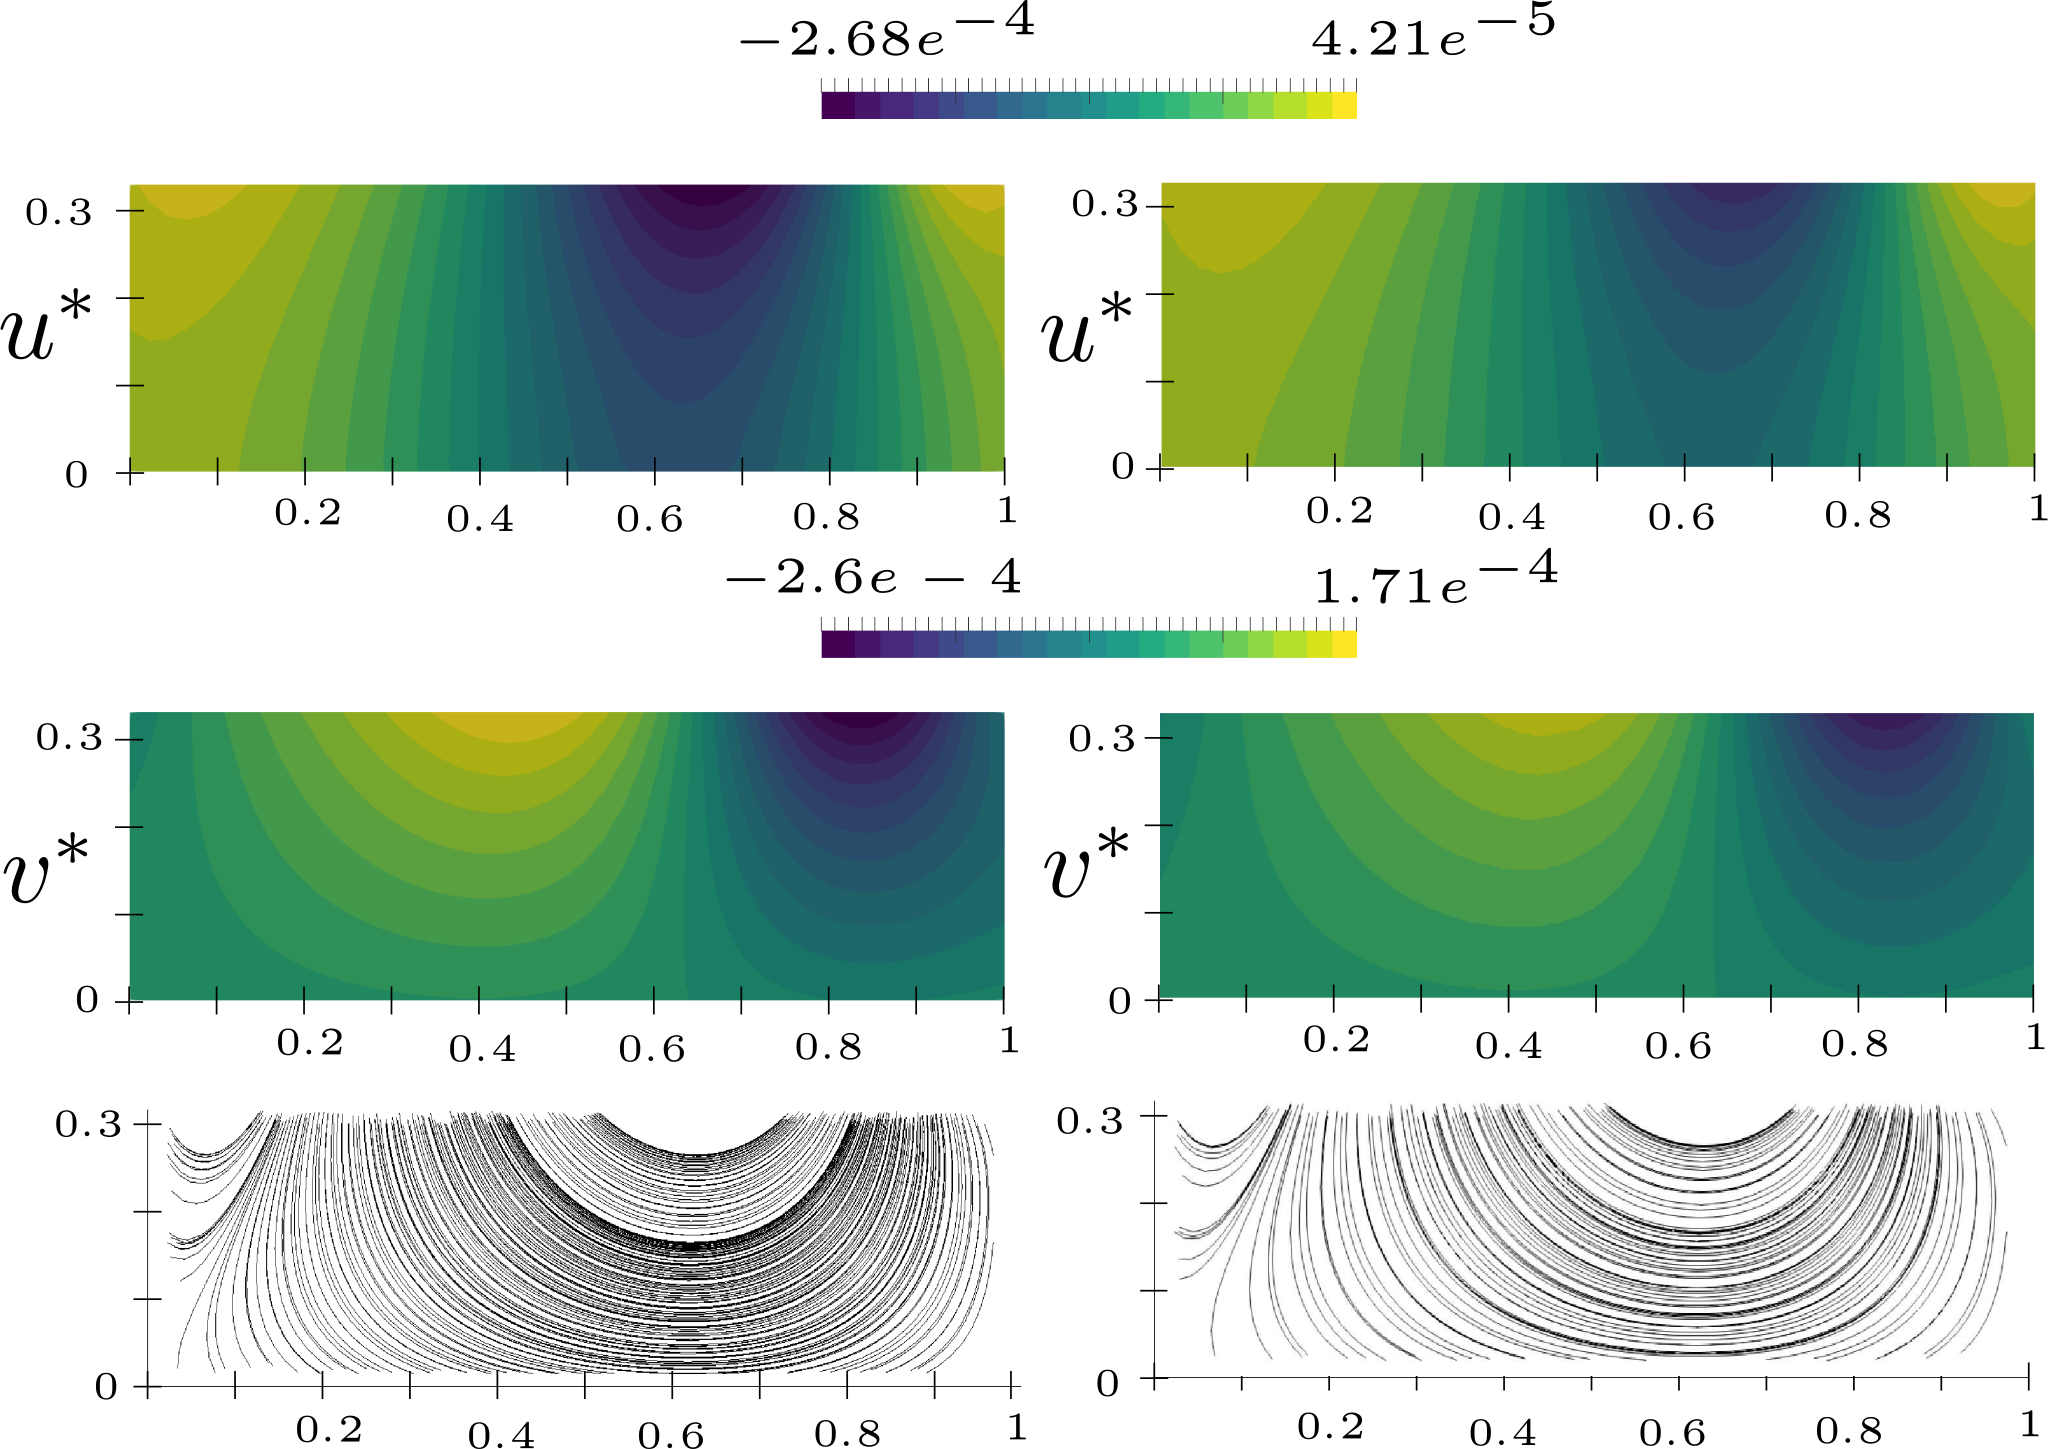
\includegraphics[width=1\linewidth]{chapter_5/figure/re100/vans_u}
	\caption{Left: VANS approach. Right: DNS approach. The figure show, from top to bottom, the horizontal velocity the vertical velocity and the streamlines inside the porous domain $\Omega_p$}
	\label{fig:100_u}
\end{figure}

\begin{figure}[h]
	\centering
	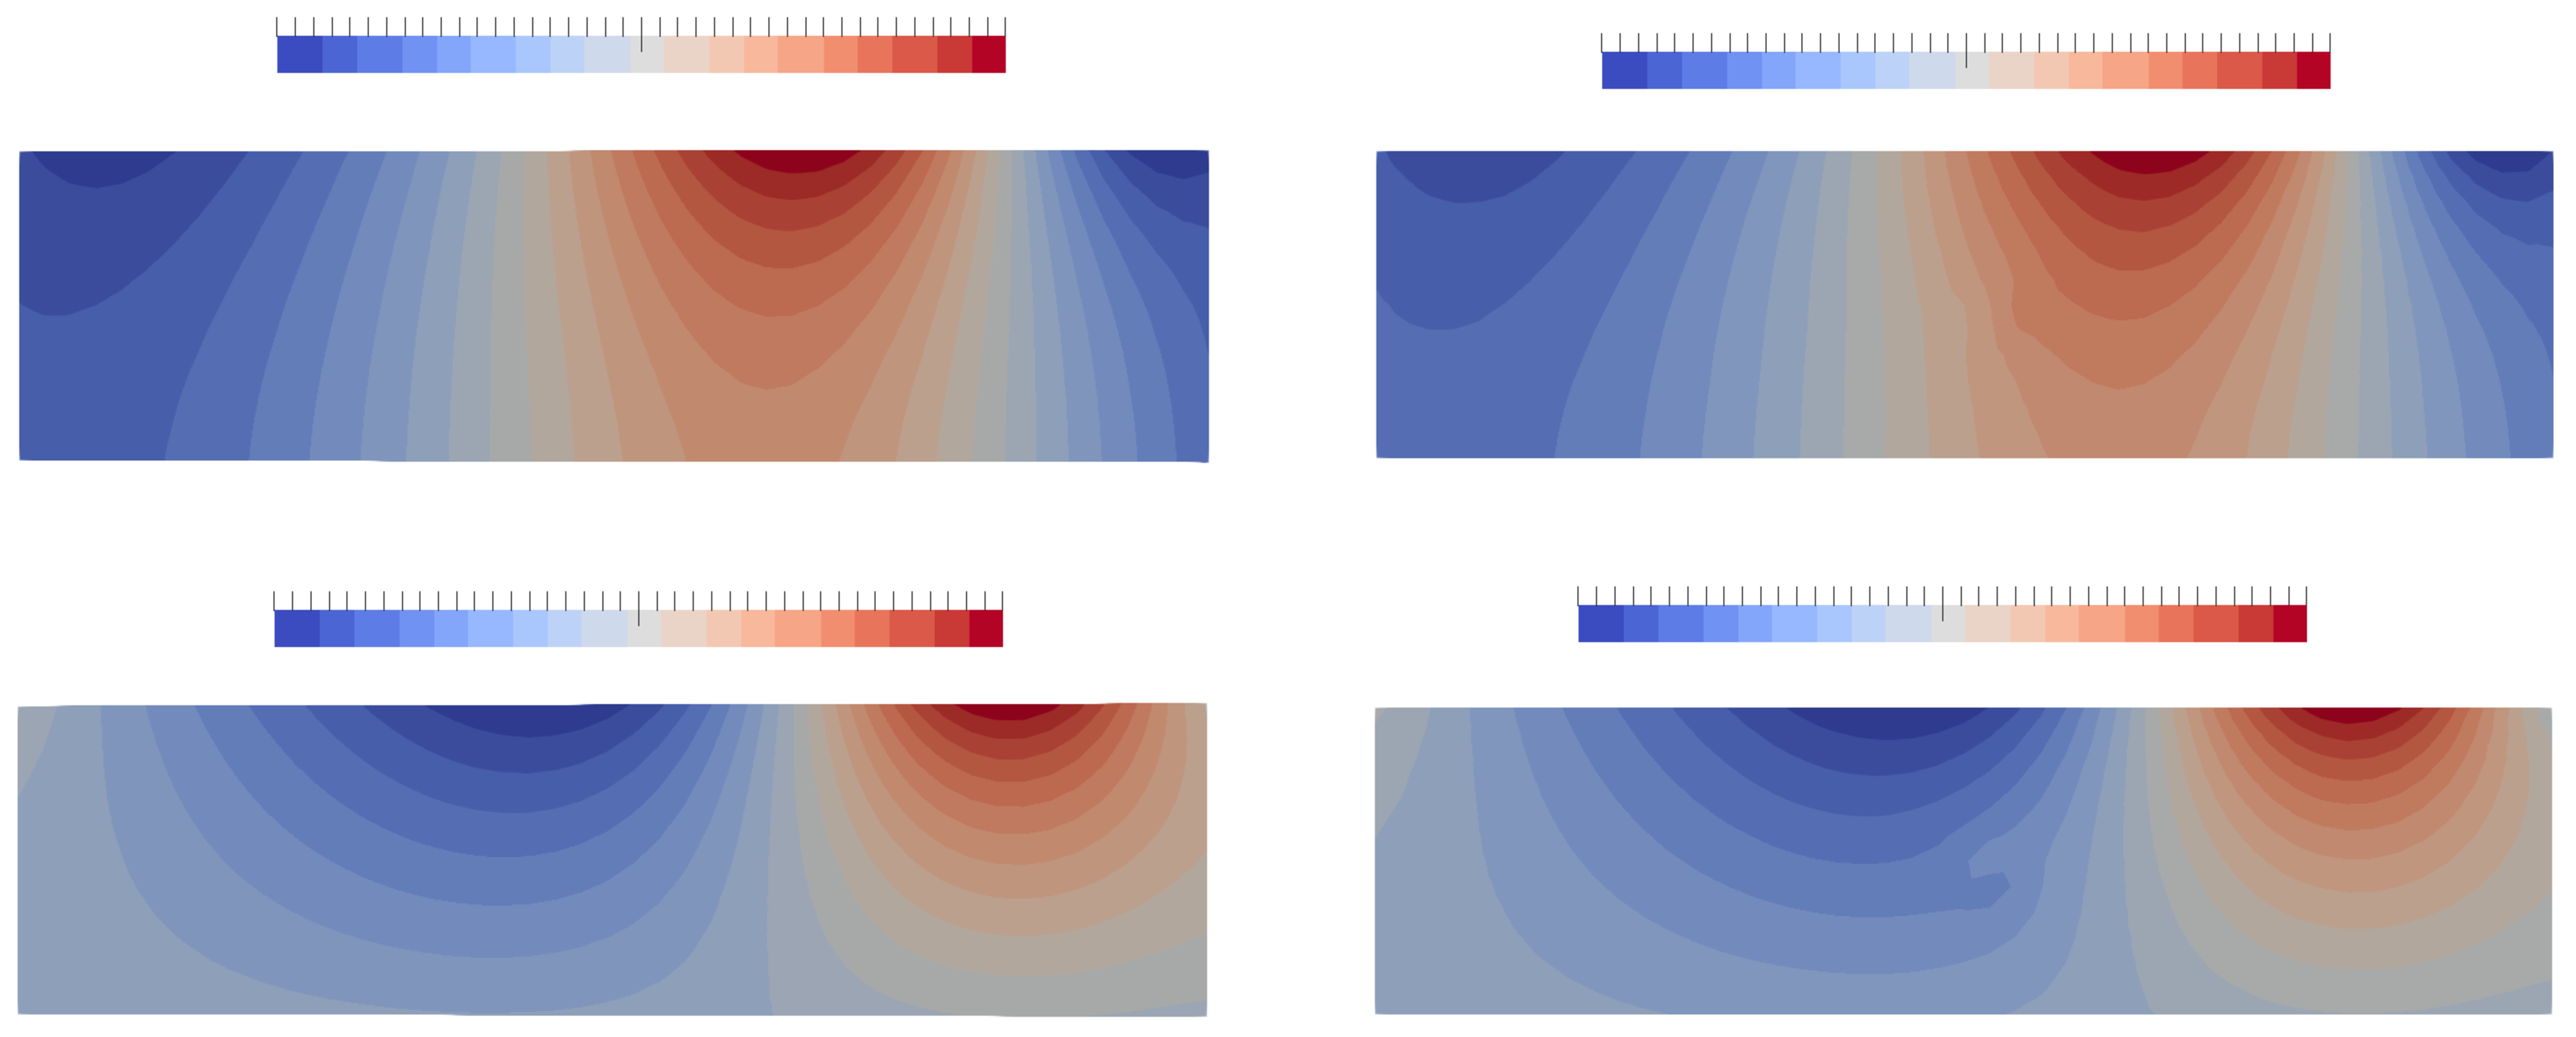
\includegraphics[width=1\linewidth]{chapter_5/figure/re100/vans_p}
	\caption{Left: VANS approach. Right: DNS approach. The figure show, from top to bottom, the horizontal and the vertical component of the pressure gradient inside the porous domain $\Omega_p$}
	\label{fig:100_p}
\end{figure}


\subsection{Cavity $Re=1000$ Comparison}

This section will present the comparison between the two different approach at $Re=1000$.
Almost the same conclusion can be gathered for this case compared to the previous one.

\begin{figure}[h]
	\centering
	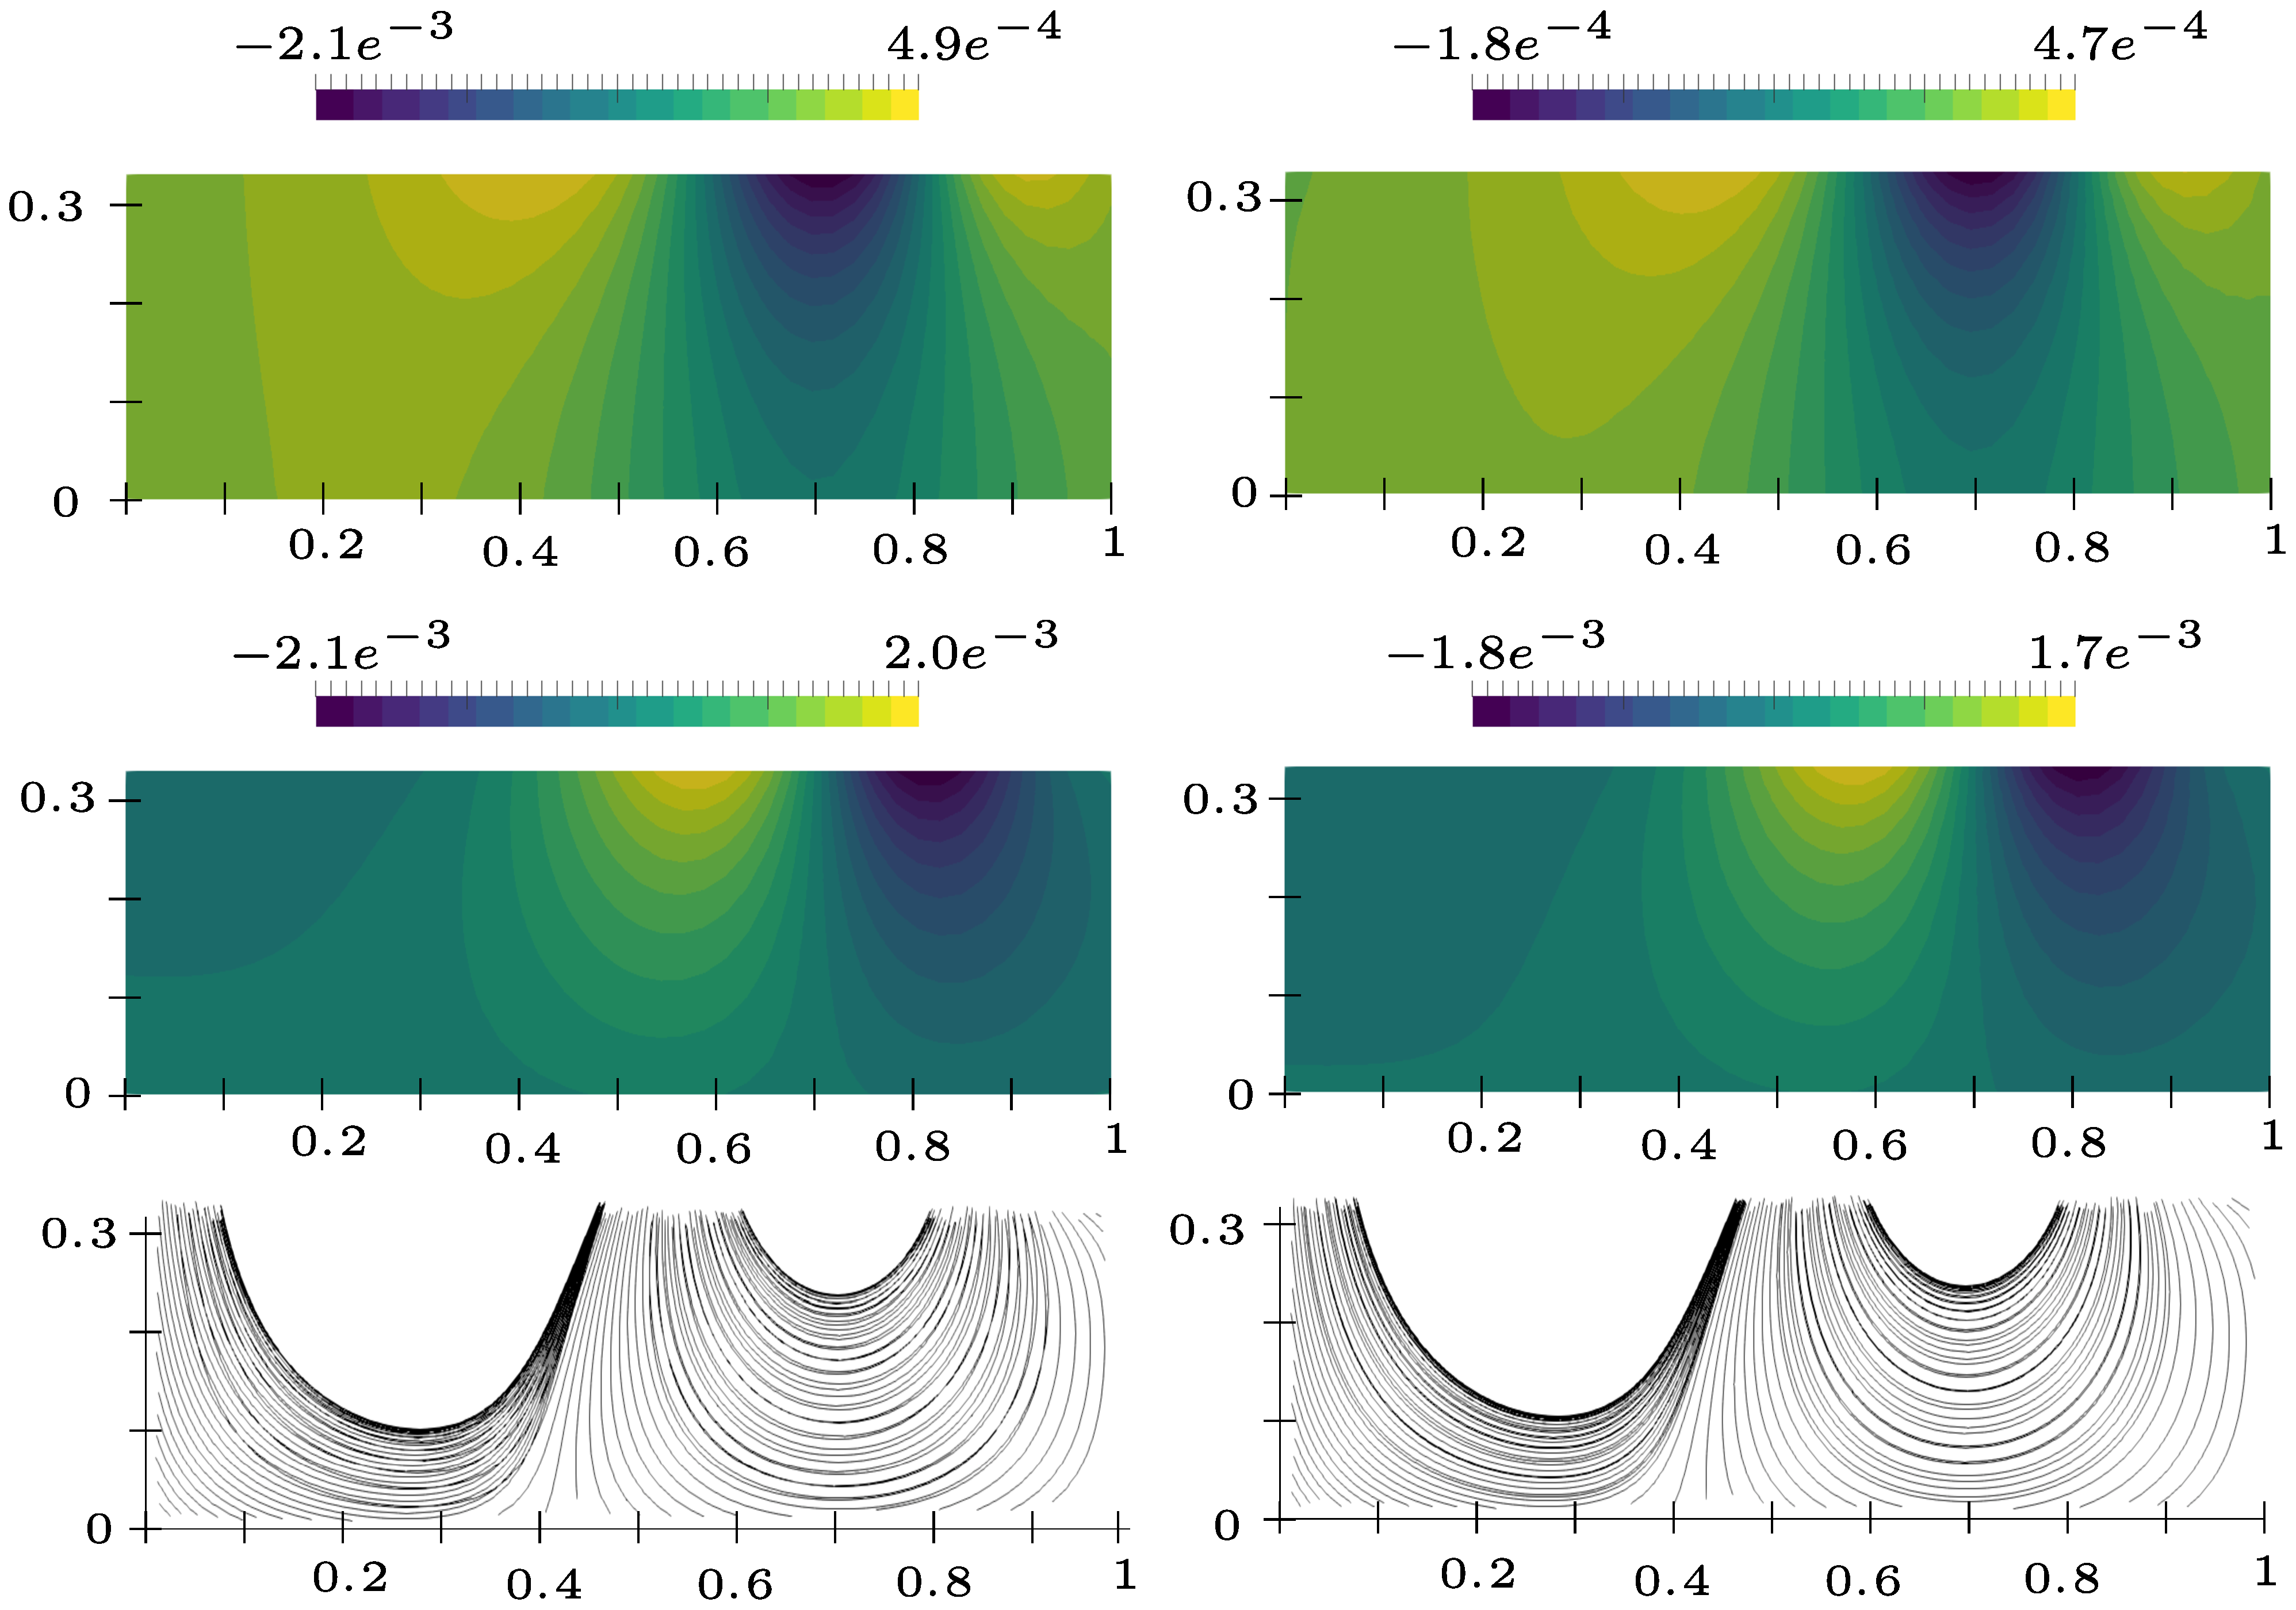
\includegraphics[width=1\linewidth]{chapter_5/figure/re1000/vans_u}
	\caption{Left: VANS approach. Right: DNS approach. The figure show, from top to bottom, the horizontal velocity the vertical velocity and the streamlines inside the porous domain $\Omega_p$}
	\label{fig:1000_u}
\end{figure}

\begin{figure}[h]
	\centering
	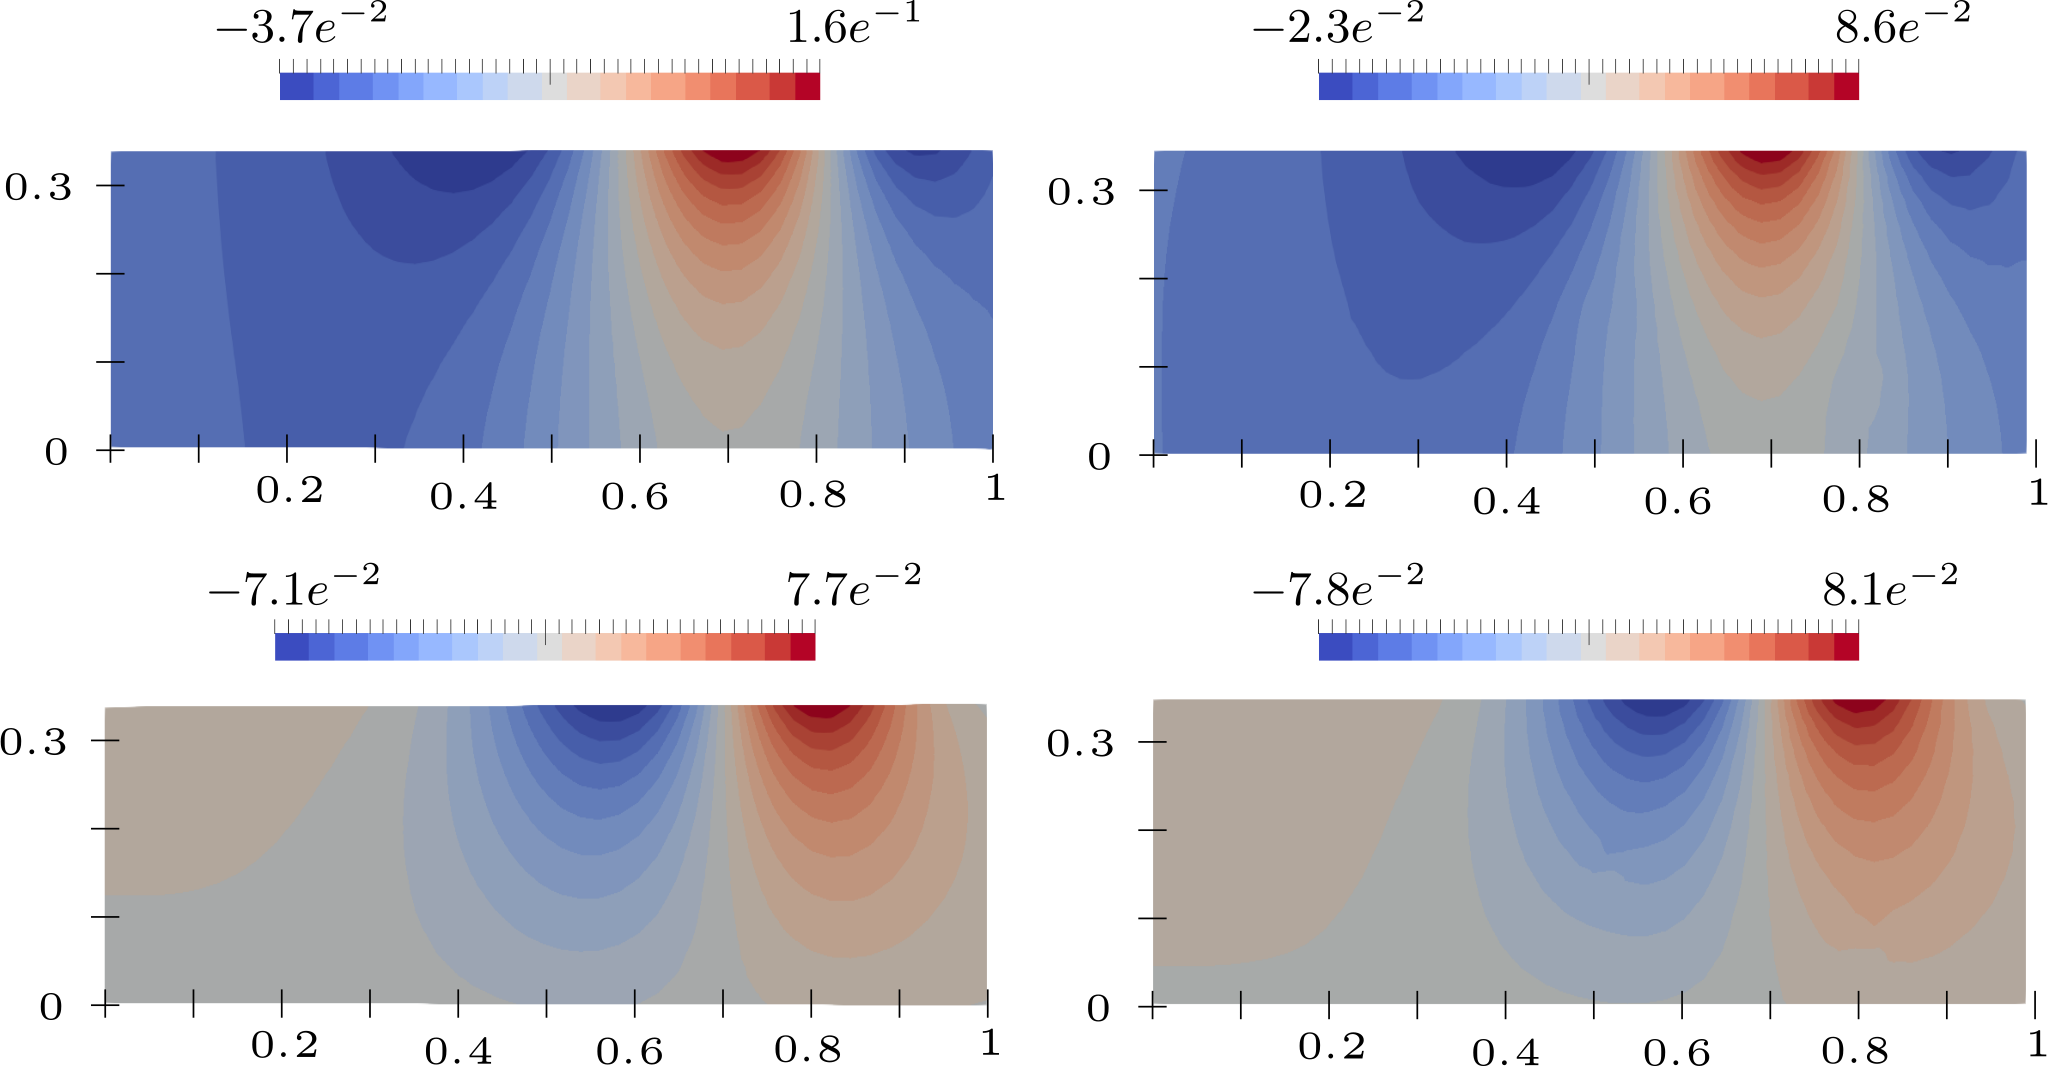
\includegraphics[width=1\linewidth]{chapter_5/figure/re1000/vans_p}
	\caption{Left: VANS approach. Right: DNS approach. The figure show, from top to bottom, the horizontal and the vertical component of the pressure gradient inside the porous domain $\Omega_p$}
	\label{fig:1000_p}
\end{figure}


\section{Separated flow between hills}




\section{Conclusions}

We have stated the two different set of equation for the two different approaches with the proper boundary conditions for the case.
The DNS approach should be taken as the reference one even if some errors due to the mesh and the solution procedure can be present.
For the two Reynolds number tested we have shown that we have a fair agreement in the velocities and pressure gradients fields.
The contours and the location of the local minima and maxima are the same for the two approaches; if we look at the numerical values, for some fields the relative errors computed at the maxima ore minima are not negligible(but the slip velocity relative error are less than $5\%$ !!!!).
We should also pinpoint that in using the VANS approach we have implicitly agree to have some differences with the DNS model; because in the former case we use a model that express the micro-scale flow behavior in terms of the macro-scale flow quantities.
With all the above reflection in mind we can be positively sure that the two model show a good agreement.

If it would be possible to obtain systematically the same results with a reduced information model \footnote{like a general metamodel or a macroscopic model for porous media or a turbulence model for turbulent flow} and a full physic simulation we would be in a paradox. Basically it would means that some of the input information are redundant. This statements should be kept in mind when making analysis on the macroscopic model against the DNS.


